\chapter{RNA-seq pre-processing}
\label{cha:mcf10a-results}
\label{sec:sequencing-depth-rna}

\begin{figure}[!h]
  \centering
  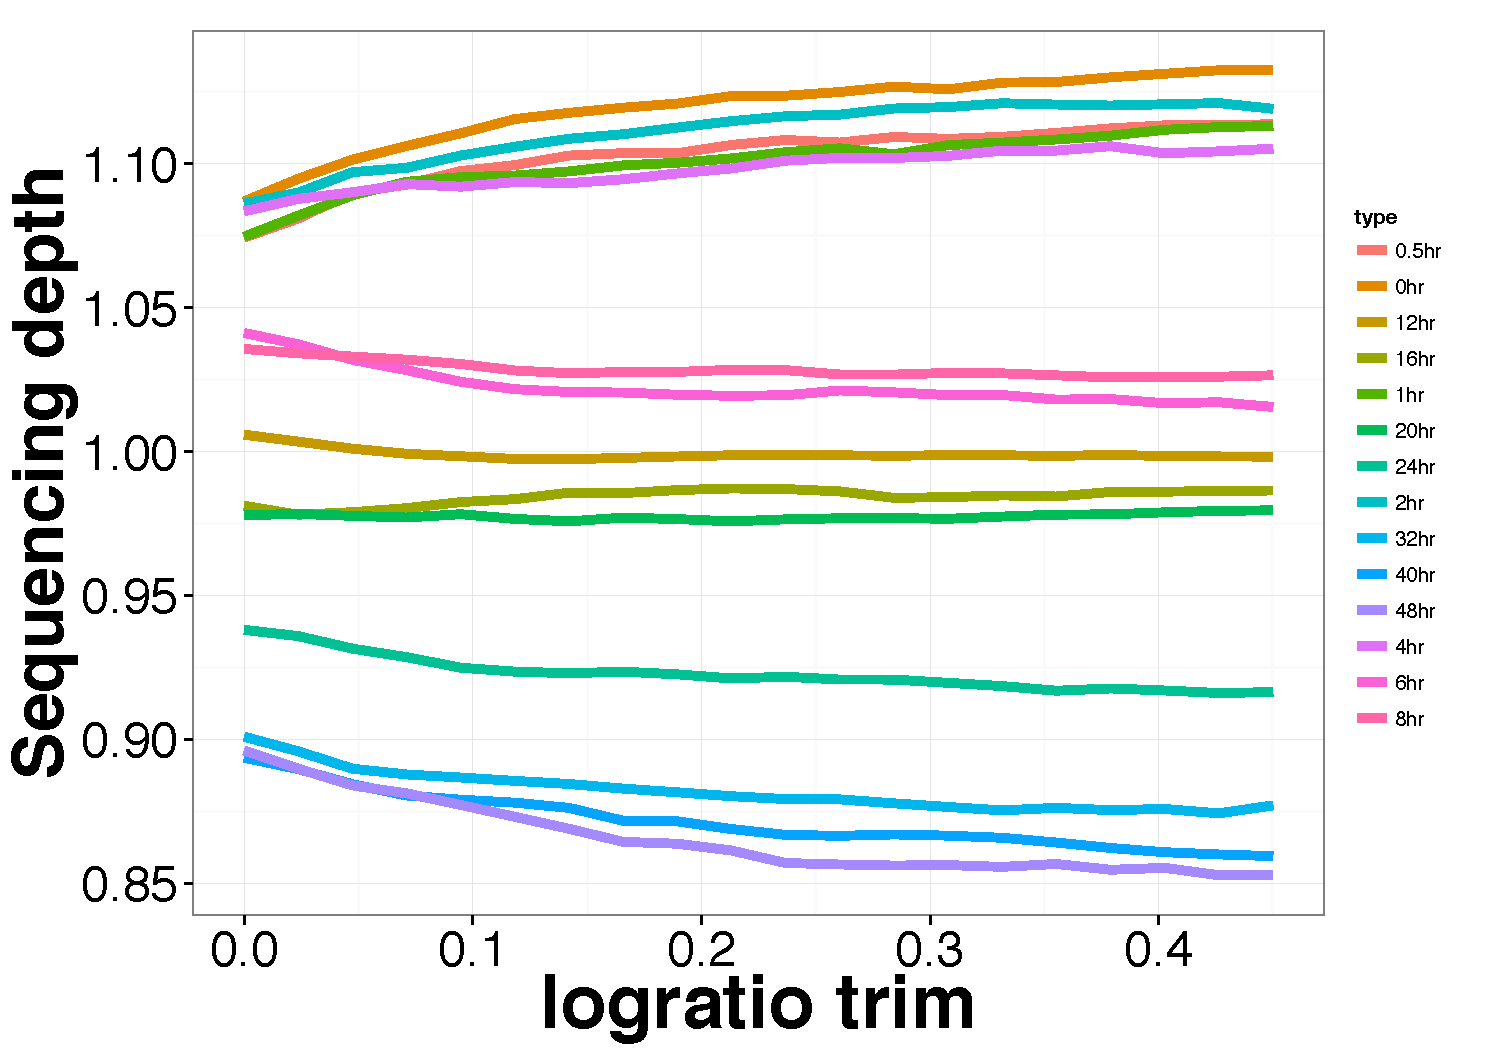
\includegraphics[width=0.8\textwidth]{pics/sequencing-depth.pdf}
  \caption{To determine sequencing depth from RNA-Seq experiments we pre-process data using the \emph{edgeR} package. See package \cite{Robinson:2010cw} for details of exact usage which briefly outlined in Section \ref{sec:normalisation}. We propose a strategy of trimming the $\log$ ratio eqn. (\ref{eq:MA-values}) at different values and identifying the cutoff that stabilises sequencing depths for the different samples. For this example we chose $0.4$.}
  \label{fig:seq-depth}
\end{figure}

%%% Local Variables:
%%% TeX-master: "warwickthesis"
%%% End:
